%%%%%%%%%%%%%%%%%%%%%%%%%%%%%%%%%%%%%%%%%%%%%%%%%%%%%%%%%%%%%%%%%%%%%%
% How to use writeLaTeX: 
%
% You edit the source code here on the left, and the preview on the
% right shows you the result within a few seconds.
%
% Bookmark this page and share the URL with your co-authors. They can
% edit at the same time!
%
% You can upload figures, bibliographies, custom classes and
% styles using the files menu.
%
%%%%%%%%%%%%%%%%%%%%%%%%%%%%%%%%%%%%%%%%%%%%%%%%%%%%%%%%%%%%%%%%%%%%%%

\documentclass[12pt]{article}
\usepackage{adjustbox}
\usepackage{sbc-template}
\usepackage{todonotes}
\usepackage{graphicx,url}
\usepackage{amsmath}
\usepackage{multirow}
\usepackage[utf8]{inputenc}  
\usepackage{babel}
\usepackage[T1]{fontenc}
\usepackage{xspace}
\usepackage{url}
\usepackage{graphicx}
\usepackage{subfig}
%----------
\usepackage{unicode-math}
\usepackage{babel}
\babeltags{br = brazil, en = english}
\usepackage[T1]{fontenc}
\usepackage{xspace}
\usepackage{url}
\usepackage{lipsum} 
%\setmathfont{xits-math.otf}
\usepackage{enumerate}
%\setmathfont[math-style=upright,range={`e,`i}]{xits-math.otf}

%--------------
\sloppy

\title{Calculo Numérico\\Trabalho\_2}


\author{Prof. Dra. Larissa de Freitas \inst{1},\\Guilherme de Souza\inst{1}}

\begin{document} 

\maketitle
\br
%\section{Funções}
%\begin{eqnarray}
%$\lambda x: 5x^{3} - 2x^{2} + 8x - 10$\\
%$\lambda x: 2x^{3} + 5x^{2} + \sin x - 30$\\
%$\lambda x: e^{-x2}\cos x$\\
%    $\lambda x: (x+1)(x-1)(x-3)^{5}\\
%    $\lambda x: (x+2)^{3}\sqrt{x^{2}+1}$
%\end{eqnarray}

\section{Métodos implementados}
\begin{itemize}
  \item Eliminação de Gauss;
  \item Fatoração LU;
  \item Cholesky;
  \item Gauss-Jabobi;
  \item Gauss-Seidel;
  \item Newton.
\end{itemize}

Para execução de tais métodos como, \textbf{Eliminação de Gauss, fatoração LU e Cholesky} foram aplicados na lista de exercícios 6\footnote{Disponivel no AVA:\url{https://ava.ufpel.edu.br/pre/pluginfile.php/313345/mod_resource/content/1/ListaDeExercicios6.pdf}}. Os métodos de \textbf{Gauss-Jacobi} e \textbf{Gauss-Seidel} utilizou-se a lista de exercícios 5\footnote{Disponivel no AVA:\url{https://ava.ufpel.edu.br/pre/pluginfile.php/312500/mod_resource/content/1/ListaDeExercicios5.pdf}}. E por ultimo na lista de exercício 7\footnote{Disponivel no AVA:\url{https://ava.ufpel.edu.br/pre/pluginfile.php/313753/mod_resource/content/1/ListaDeExercicios7.pdf}}.


\section{Eliminação de Gauss}

Nesta seção é apresentado o método de \textit{Eleminição de Gauss}, é uma técnica para simplificar a resolução de sistemas lineares como:

\begin{cases}
2x-5y+z=1 \\
3x-y+2z=3 \\
4x-y-3z=-1
\end{cases}

O sistema linear acima conta com três icógnitas e, descobrir seus valores pode ser dificil ou em alguns casos impraticavel, mas fazendo uso do método se torna mais simples sua resolução. O método conta com três teoremas: 

\begin{enumerate}[i]
   \item O sistema de equações não se altera quando permutamos as posições das equações;
   \item O sistema de equações não se altera quando multiplicamos os membros de uma das equações por qualquer número real não nulo;
   \item Por inferência, podemos então substituir uma equação por outra obtida a partir da inclusão “membro a membro” desta equação, por outra na qual foi aplicada a transformação do Teorema 2 acima.
 \end{enumerate}

Para encontrar a resolução apartir do método, tem por objetivo fazer uso dos teoremas para conseguir zerar duas das três icógnitas de uma das linhas, a fim de poder determinar a icógnita que restar, assim partindo dela poder resolver o restante do sistema substituindo termo a termo.

O método foi implementado em python como pedido pela disciplina e executado em cima de uma lista de exercícios. Com isso, é demonstrado a seguir quatro matrizes derivadas dos sistemas das listas e suas respectivas resolução após a execução do método. É apresentado na Tabela 1 a Tabela 12 as matrizes de entrada, as resultantes após a aplicação do método e os resultados encontrados para as icógnitas.

%---------------------------------------------------------------------------------------------------
% MATRIZ NUMERO 1
%---------------------------------------------------------------------------------------------------
\begin{table}[htb]
  \begin{minipage}[b]{.46\linewidth}

    \centering
    \begin{tabular}{|c c c|c|}
        -2           &          3           &          1      &   -5 \\
        2           &          1           &          -4      &   -9 \\
        7           &          10           &          -6     &   2 \\
    \end{tabular}
    \caption{Matriz de entrada 1}
    \label{tab:esq}

  \end{minipage}\hfill
  \begin{minipage}[b]{.46\linewidth}

    \centering
    \begin{tabular}{|c c c|c|}
        7           &          10           &          -6      &   2 \\
        0           &          5           &          0      &   -4 \\
        0           &          0           &          -2     &   -9 \\
    \end{tabular}
    \caption{Matriz resultante 1}
    \label{tab:dir}
  \end{minipage}
\end{table}


\begin{table}[!h]
\centering
\begin{tabular}{|l|}
\multicolumn{1}{|c|}{5.2857} \\
-0.8                         \\
4.5                         
\end{tabular}
\caption{Resultado matriz 1}
\end{table}

%---------------------------------------------------------------------------------------------------
% MATRIZ DOIS
%---------------------------------------------------------------------------------------------------

\begin{table}[htb]
  \begin{minipage}[b]{.46\linewidth}

    \centering
    \begin{tabular}{|c c c c|c|}
        1           &         -3          &           5     &   6     &   17\\
        -9          &         4           &          -1     &   0     &   29\\
        3           &         2           &          -2     &   7     &   -11\\
        1           &         2           &           5     &   -4    &   7\\
    \end{tabular}
    \caption{Matriz de entrada 2}
    \label{tab:esq}

  \end{minipage}\hfill
  \begin{minipage}[b]{.46\linewidth}

    \centering
    \begin{tabular}{|c c c c|c|}
        -9           &         4          &           -1     &   0     &   29\\
        0          &         3           &          -2     &   7     &   -1\\
        0           &         0           &          5     &   -8     &   10\\
        0           &         0           &           0     &   13    &   15\\
    \end{tabular}
    \caption{Matriz resultante 2}
    \label{tab:dir}
  \end{minipage}
\end{table}


\begin{table}[!h]
\centering
\begin{tabular}{|l|}
\multicolumn{1}{|c|}{-3.8547} \\
-0.4615                         \\
3.8462                        \\
1.1538
\end{tabular}
\caption{Resultado matriz 2}
\end{table}

%---------------------------------------------------------------------------------------------------
% MATRIZ 3
%---------------------------------------------------------------------------------------------------
\begin{table}[htb]
  \begin{minipage}[b]{.46\linewidth}

    \centering
    \begin{tabular}{|c c c c|c|}
        -2           &         3          &           1     &   5     &   2\\
        5          &         1           &          -1     &   0     &   -1\\
        1           &         6           &          3     &   -1     &   0\\
        4          &         5           &           2     &   8    &   6\\
    \end{tabular}
    \caption{Matriz de entrada 3}
    \label{tab:esq}

  \end{minipage}\hfill
  \begin{minipage}[b]{.46\linewidth}

    \centering
    \begin{tabular}{|c c c c|c|}
        5           &         1          &           -1     &   0     &   -1\\
        0          &         5           &          3     &   -1     &   0\\
        0           &         0           &          -1     &   5     &   1\\
        0           &         0           &           0     &   8    &   6\\
    \end{tabular}
    \caption{Matriz resultante 3}
    \label{tab:dir}
  \end{minipage}
\end{table}


\begin{table}[!h]
\centering
\begin{tabular}{|l|}
\multicolumn{1}{|c|}{0.65} \\
-1.5                         \\
3.75                        \\
0.75
\end{tabular}
\caption{Resultado matriz 3}
\end{table}

%---------------------------------------------------------------------------------------------------
% MATRIZ 4
%---------------------------------------------------------------------------------------------------
\begin{table}[htb]
  \begin{minipage}[b]{.46\linewidth}

    \centering
    \begin{tabular}{|c c c c c|c|}
        0           &         1          &           3     &   2     &   4   &   3\\
        8          &         -2           &          9     &   -1     &   2   &   -5\\
        5           &         1           &          1     &   7     &   2   &   6\\
        -2          &         4           &           5     &   1    &     0   &   -1\\
        7          &         -3           &           2     &   -4    &     1   &   8\\
    \end{tabular}
    \caption{Matriz de entrada 4}
    \label{tab:esq}

  \end{minipage}\hfill
  \begin{minipage}[b]{.46\linewidth}

    \centering
    \begin{tabular}{|c c c c c|c|}
        8           &         -2          &           9     &   -1     &   2   &   -5\\
        0          &         3           &          7     &   0     &   0   &   -2\\
        0           &         0           &          -8     &   7     &   0   &   10\\
        0          &         0           &           0     &   -4    &     0   &   8\\
        0          &         0           &           0     &   0    &     4   &   7\\
    \end{tabular}
    \caption{Matriz resultante 4}
    \label{tab:dir}
  \end{minipage}
\end{table}


\begin{table}[!h]
\centering
\begin{tabular}{|l|}
\multicolumn{1}{|c|}{3.6458} \\
6.3333                         \\
-3                        \\
-2                        \\
1.75
\end{tabular}
\caption{Resultado matriz 4}
\end{table}

Podemos observar que o resultado das icógnitas é apresentado mantendo a mantissa em quatro digitos, para melhor visualização, o mesmo faz uso de arredontamento. O resultado é apresentado em modelo de coluna seguindo o seguinte padrão:

\left[ \begin{array}{c}
x \\
y \\
z 
\end{array} \right]

\section{Fatoração LU}

Neste métodos realizamos uma operação um pouco diferente da multiplicação de matrizes. Antes tinhamos \textit{AB=C} agora realização a fatoração da mesma, ou seja, \textit{C=AB}, partiremos de da matriz C e encontraremos as matrizes A e B.

Esse método é interessante pelo fato de que usaremos um computador para computar essa quantidade de matrizes, dado um computador qualquer ele realiza X operações por segundo e, queremos que ele realize menos operações possiveis, dessa forma, vou estar gastando menos tempo. Seguindo o pessamento se temos \textit{Ax=b} para solucionar teremos que \textit{x=inversa(A)b}.E realizar isso um milhão de vezes é muito custoso, até mesmo para maquinas.

Com isso realizando a fatoração LU, teremos ao invés de \textit{Ax=b}, \textit{LUx=b}. Dessa forma estaremos realizando por partes nosso problema, de forma a reduzir o número de operações ates realizados e, assim reduzimos o tempo.

Para aplicação desse métodos basta seguir um simples algoritimo\footnote{Créditos do algoritimo ao MeSalva:\url{https://www.youtube.com/watch?v=6VBdlqrS2yU}}
\begin{enumerate}[i]
   \item Escalone A até achar U;
   \item As colunas de L serão encontradas durante o escalonamento (apenas colunas LI);
   \item Se A possui mais colunas que linhas, as colunas de L são iguais a I.
 \end{enumerate}

Para visualização do método, o mesmo foi aplicado a sua lista destinada, os resultados podem ser vistos na Tabela 13 à tabela 21.

%---------------------------------------------------------------------------------------------------
% MATRIZ 1
%---------------------------------------------------------------------------------------------------
\begin{table}[!ht]
  \begin{minipage}[b]{.46\linewidth}

    \centering
    \begin{tabular}{|c c c|c|}
        1           &         0          &           0     &   0\\
        0.25           &         1          &           0     &   0\\
        1.25           &         1          &           1     &   0\\
        0.5           &         0.6667          &           1     &   1\\
    \end{tabular}
    \caption{Matriz LU 1}
    \label{tab:dir}

  \end{minipage}\hfill
  \begin{minipage}[b]{.46\linewidth}

    \centering
    \begin{tabular}{|c c c|c|}
        4           &         -1          &           3     &   8\\
        0           &         6          &           1     &   -5\\
        0           &         0          &           -3     &   -5\\
        0           &         0          &           0     &   5\\
    \end{tabular}
    \caption{Matriz U 1}
    \label{tab:esq}

  \end{minipage}\hfill
  \begin{minipage}[b]{.46\linewidth}

    \centering
    \begin{tabular}{|c|}
        -3\\
        4\\
        4\\
        6\\
    \end{tabular}
    \caption{Resolução Matriz 1}
    \label{tab:dir}
  \end{minipage}
\end{table}


%---------------------------------------------------------------------------------------------------
% MATRIZ 2
%---------------------------------------------------------------------------------------------------
\begin{table}[!ht]
  \begin{minipage}[b]{.36\linewidth}

    \centering
    \begin{tabular}{|c c c c c|}
        1                 &         0                   &           0             &   0     &   0   \\
        -0.33333          &         1                   &          0               &   0     &   0   \\
        2.66667           &         27.99946           &          1                &   0     &   0   \\
        0.66667          &         -4.99988           &           -0.21978          &   1    &     0  \\
        -0.33333          &         6.99988           &           0.26027           &   0.17222    &     1\\
    \end{tabular}
    \caption{Matriz LU 2}
    \label{tab:dir}


  \end{minipage}\hfill
  \begin{minipage}[b]{.46\linewidth}

    \centering
    \begin{tabular}{|c|}
        -68\\
        28\\
        280\\
        -72\\
        362\\
    \end{tabular}
    \caption{Resolução Matriz 2}
    \label{tab:dir}
  \end{minipage}\hfill
  \begin{minipage}[b]{.36\linewidth}

    \centering
    \begin{tabular}{|c c c c c|}
        3                 &         -2       &           -1             &   7     &   3   \\
        0          &         0.33334          &          2.66667        &   0.33331     &   -2.00001   \\
        0           &         0               &          -72.99865      &   -27.99919     &   49.99919   \\
        0          &         0                &           0             &   -4.13704    &     -1.041\\
        0          &         0                &           0             &   0    &     0.16581\\
    \end{tabular}
      \caption{Matriz U 2}
    \label{tab:esq}
  \end{minipage}

\end{table}

%---------------------------------------------------------------------------------------------------
% MATRIZ 3
%---------------------------------------------------------------------------------------------------

\begin{table}[!h]
    \centering
    \begin{tabular}{|c c c c c c|}
        1           &         0          &           0                        &   0             &   0      &   0\\
        0.25          &         1           &          0                      &   0             &   0      &   0\\
        -0.5           &         -1.66666667           &          1           &   0             &   0     &   0\\
        1.75           &         4           &           -2.03743315          &   1             &   0       &   0\\
        2.5           &         3.83333333           &           -2.133636363 &   0.27928898    &   1       &   0\\
        2           &         2.33333333           &           -1.53475936    &   0.6587665    &   -1.9408528       &   1\\
    \end{tabular}
    \caption{Matriz L 3}
    \label{tab:esq}
\end{table}

\begin{table}[!h]
    \centering
    \begin{tabular}{|c c c c c c|}
        4           &         12          &           14                        &   5             &   2      &   -1\\
        0          &         -6           &          8.5                      &   0.75             &   2.5      &   -1.75\\
        0           &       0           &          31.1666667           &   4.75             &   3.166666666     &   -3.41666667\\
        0           &         0           &           0          &   9.92780746             &   0.95187167       &   11.78877006\\
        0           &         0           &           0 &   0    &   3.91597093       &   -9.38338265\\
        0           &       0           &           0    &   0    &   0       &   -10.1382391\\
    \end{tabular}
    \caption{Matriz U 3}
    \label{tab:dir}
\end{table}

\begin{table}[!h]
    \centering
    \begin{tabular}{|c|}
        23\\
        11\\
        14\\
        -80\\
        66\\
        41\\
    \end{tabular}
    \caption{Resolução Matriz 3}
    \label{tab:dir}
\end{table}


Apresentando os resultados como  a matriz L, matriz U e a solução para seu respectivo sistema, sendo o resultado apresentado da mesma forma que na seção anterior. Em cada aplicação dos métodos fez-se uso de tamanho de mantissas diferentes seguindo 4, 5 e 8 respectivamente em cada matriz, podendo analizar que temos uma aproximação maior dado um maior numero de cassas decimais.

\section{Cholesky}

Seguindo a mesma idéia em ganho de eficiência como no método anterior apresentado, o método de cholesky tem por objetivo decompor A em G$G^{T}$ desde que sua matriz seja positiva definida. Assim teremos uma matriz triangular inferior e sua matriz adjunta. Esse método é comumente usado para simulações de Monte Carlo, ja demonstrado ser duas vezes mais eficiênte que a fatoração LU. Os resultados podem ser visto a seguir, obervando as Tabelas 22 a 30.
%--------------------------------------------------------------------------------------------------------------------------------
%    MATRIZ 1
%--------------------------------------------------------------------------------------------------------------------------------

\begin{table}[!ht]
  \begin{minipage}[b]{.36\linewidth}

    \centering
    \begin{tabular}{|c c c|}
        3                 &         0                   &           0    \\
        -2          &         5                   &          0  \\
        1           &         -1           &          4    \\
    \end{tabular}
    \caption{Matriz G 1}
    \label{tab:dir}


  \end{minipage}\hfill
  \begin{minipage}[b]{.46\linewidth}

    \centering
    \begin{tabular}{|c|}
        -1\\
        0\\
        2\\
    \end{tabular}
    \caption{Resolução Matriz 1}
    \label{tab:dir}
  \end{minipage}\hfill
  \begin{minipage}[b]{.36\linewidth}

    \centering
    \begin{tabular}{|c c c|}
        3                 &         -2       &           1  \\
        0          &         5          &          -1       \\
        0           &         0               &          4  \\
    \end{tabular}
      \caption{Matriz GT 1}
    \label{tab:esq}
  \end{minipage}

\end{table}


%---------------------------------------------------------------------------------------------------
% MATRIZ 2
%---------------------------------------------------------------------------------------------------
\begin{table}[!ht]
  \begin{minipage}[b]{.36\linewidth}

    \centering
    \begin{tabular}{|c c c c|}
        2           &         0                   &           0             &   0     \\
        -1          &         1.41421            &          0               &   0     \\
        2           &         0.70711           &          3.08221                &   0 \\
        5          &         -1.41422            &           0          &   1.8918  \\
    \end{tabular}
    \caption{Matriz G 2}
    \label{tab:dir}


  \end{minipage}\hfill
  \begin{minipage}[b]{.46\linewidth}

    \centering
    \begin{tabular}{|c|}
        3\\
        1\\
        -0\\
        -1\\
    \end{tabular}
    \caption{Resolução Matriz 2}
    \label{tab:dir}
  \end{minipage}\hfill
  \begin{minipage}[b]{.36\linewidth}

    \centering
    \begin{tabular}{|c c c c|}
        2                 &         -1       &           2             &   5    \\
        0          &        1.41421          &          0.70711        &   -1.41422      \\
        0           &         0               &         3.08221      &   0.64889     \\
        0          &         0                &           0             &   1.8918    \\
    \end{tabular}
      \caption{Matriz GT 2}
    \label{tab:esq}
  \end{minipage}

\end{table}



%---------------------------------------------------------------------------------------------------
% MATRIZ 3
%---------------------------------------------------------------------------------------------------
\begin{table}[!ht]
  \begin{minipage}[b]{.36\linewidth}

    \centering
    \begin{tabular}{|c c c c c|}
        1&         0 &           0             &   0     &   0   \\
        2&         1&          0               &   0     &   0   \\
        -3&         5&          4                &   0     &   0   \\
        0&         1&           -1          &   2    &     0  \\
        3&         -2&           0           &   1    &     5\\
    \end{tabular}
    \caption{Matriz G 3}
    \label{tab:dir}


  \end{minipage}\hfill
  \begin{minipage}[b]{.46\linewidth}

    \centering
    \begin{tabular}{|c|}
        -2\\
        8\\
        -1\\
        4\\
        0\\
    \end{tabular}
    \caption{Resolução Matriz 3}
    \label{tab:dir}
  \end{minipage}\hfill
  \begin{minipage}[b]{.36\linewidth}

    \centering
    \begin{tabular}{|c c c c c|}
        1           &         2               &           -3             &   0     &   3   \\
        0          &         1                &          5                &   1     &   -2   \\
        0           &         0               &          4                &   -1     &   0   \\
        0          &         0                &           0             &   2    &     1\\
        0          &         0                &           0             &   0    &    5\\
    \end{tabular}
      \caption{Matriz GT 3}
    \label{tab:esq}
  \end{minipage}

\end{table}

Como na seção anterior, apresentamos os resultados igualmente, apresentando G e a $G^{T}$. Junto a solução do sistema, para esse método fez-se uso de 5 digitos para mantissa.

\section{Fatoração Gauss-Jacobi}

Aqui iniciamos a primeira seção de metodos iterativos, apresentando Gauss-Jacobi. Tais métodos podem ser mais rapidos e exigir  menos memória do computador, fornecendo sequências que convergem para soluções sob certar condições.

Dito isso, seja \textit{Ax=B} um sistema linear de ordem N. A ideia é generalizar o métodos do ponto fixo, escrevendo o sistema linear \textit{x=Cx+g}, onde C é uma matriz de ordem N e g é um vetor coluna Nx1. Dado um vetor de iteração inicial $x^{(0)}$ podemos ir construindo iterativamente. 

\begin{figure}[!h]
    \centering
    \includegraphics[scale=0.3]{/home/souza/Documents/semestre_2019-2/calculo_numerico/trabalho_2/Graficos/gauss_jacobi/1.png}
    \caption{Gráfico da função um da lista cinco executada pelo método Gauss-Jacobi.}
\end{figure}

Na Figura 1, podemos observar o resultado obtido pela execução do código. Para a primeira execução passamos o erro como 0.05 e um total máximo de iterações 4. Podemos ver que o método se apresentou um tanto quanto eficiente (olhando singularmente), porém o mesmo só irá convergir  em  7 iterações.

\begin{figure}[!h]
    \centering
    \includegraphics[scale=0.3]{/home/souza/Documents/semestre_2019-2/calculo_numerico/trabalho_2/Graficos/gauss_jacobi/2.png}
    \caption{Gráfico da função dois da lista cinco executada pelo Gauss-Jacobi.}
\end{figure}

Na Figura 2, segui fazendo uso do 0.05 como erro e, para quatro para numero de máximo de iterações, porém testes com numeros mariores foram executados para comprovação de uma convergência a longo prazo, porém o sistema não converge.

\begin{figure}[!h]
    \centering
    \includegraphics[scale=0.3]{/home/souza/Documents/semestre_2019-2/calculo_numerico/trabalho_2/Graficos/gauss_jacobi/3.png}
    \caption{Gráfico da função três da lista cinco executada pelo método Gauss-Jacobi.}
\end{figure}

Na Figura 3, segue os mesmo parâmetros, testes com maior numero de iterações foram executados, para comprovação de uma convergência em 750 iterações, porém por padronização seguimos com 4 iterações.

\begin{figure}[!h]
    \centering
    \includegraphics[scale=0.3]{/home/souza/Documents/semestre_2019-2/calculo_numerico/trabalho_2/Graficos/gauss_jacobi/4.png}
    \caption{Gráfico da função um da lista cinco executada pelo método Gauss-Jacobi.}
\end{figure}

Seguindo na Figura 4, os mesmo parametros se sucedem, erro em 0.05 e numero de iterações máxima em 4. Neste sistema voltamos a convergir com um numero ainda menor que anteriormente, levando somente 4 iterações.

\section{Fatoração Gauss-Seidel}

Assim como na seção anterior, seguimos com métodos iterativos, o Gauss-Seidel é semelhante ao de Jacobi, seguindo os mesmos critérios para convergência. Neste método é condição suficiente que a matriz seja extritamente diagonal dominante, com isso fica garantido a convergência da sucessão de valores gerados para solução exata do sistema.

Com isso esse método acaba por convergir mais rapido que o Jacobi, isso pode ver visto de acordo com os resultados apresentados a seguir.

\begin{figure}[!h]
    \centering
    \includegraphics[scale=0.3]{/home/souza/Documents/semestre_2019-2/calculo_numerico/trabalho_2/Graficos/gauss_seidel/1.png}
    \caption{Gráfico da função um da lista cinco executada pelo método Gauss-Seidel.}
\end{figure}

Na Figura 5 temos como parâmetro de entrada valores parecidos com os do método anterior, erro em 0.05 e numero máximo de iterações em 4. Podemos observar que apenas em quatro iterações o método ja convergiu, enquanto no método anterior precisou-se de 7, ou seja, o método realmente se demonstra mais "rapido" que o anterior.

\begin{figure}[!h]
    \centering
    \includegraphics[scale=0.3]{/home/souza/Documents/semestre_2019-2/calculo_numerico/trabalho_2/Graficos/gauss_seidel/2.png}
    \caption{Gráfico da função dois da lista cinco executada pelo método Gauss-Seidel.}
\end{figure}

Na Figura 6 ja podemos começar a notar a distância entre os pontos, levando as quatro iterações e ainda sim não convergindo como o anterior. Um maior numero de iterações foi passados para fim de teste de convergência, porém o mesmo segue a não convergir mesmo em 1000 iterações.

\begin{figure}[!h]
    \centering
    \includegraphics[scale=0.3]{/home/souza/Documents/semestre_2019-2/calculo_numerico/trabalho_2/Graficos/gauss_seidel/3.png}
    \caption{Gráfico da função três da lista cinco executada pelo método Gauss-Seidel.}
\end{figure}

Na Figura 7, encontramos um resultado semelhante com a 6, não convergindo ao final das iterações, e com uma grafico com pontos extremamente distântes.

\begin{figure}[!h]
    \centering
    \includegraphics[scale=0.3]{/home/souza/Documents/semestre_2019-2/calculo_numerico/trabalho_2/Graficos/gauss_seidel/4.png}
    \caption{Gráfico da função um da lista cinco executada pelo método Gauss-Seidel.}
\end{figure}

Analisando a Figura 8, notamos que voltamos a converir, só que agora com um numero ainda menor que o anterior, convergindo em somente 3 iterações, podemos notar que gráficos que convergem, tendem seus pontos ficarem proximos, quanto aos que não convergem, mantem uma certa distância entre eles, isso é notavel na aplicação deste método, bastando analisar os gráficos.

\section{Newton}

O método de Newton tem por objetivo resolver equações não lineares (observe que estou falando desse método em específico, dado que equação de Newton com algumas alterações tem outros objetivos), assim, consiste em dada uma aproximação inicial $x^{0}$ da solução, calcular a aproximação (formula ocultada), a cada iteração k $\geq$ 0, até que o critério de convergência seja satisfeito, que na minha minha implementação é dado pelo erro e numero iterações.

Como aproximação inicial foi passado para o primeiro sistema [1, 2, 3], erro 0.001 e numero de iteração máxima 4. Para as demais fez-se uso dos mesmo parâmetros, somente alterando a aproximação inicial para [1, 2]. Para os sistemas passado em lista fora encontrado as respectivas soluções, sera aprensentado em cada iteração, observando as Tabelas 31 a 34.

\begin{table}[!ht]
    \centering
\begin{tabular}{|lll|}
\multicolumn{1}{|c}{-2.62886598} & 8.04123711 & 3.04123711 \\
-2.37227892                      & 4.06823601 & 1.7994454  \\
-2.99221917                      & 1.75082435 & 0.55478453 \\
-1.18759971                      & 1.38106959 & 0.45175715
\end{tabular}
    \caption{Solução do exercício A aplicando Newton.}
\end{table}

\begin{table}[!ht]
    \centering
\begin{tabular}{|ll|}
\multicolumn{1}{|c}{0.45614035} & 1.05263158 \\
0.15361382                      & 0.54118776 \\
-0.03869295                     & 0.27367009 \\
0.13379586                      & 0.13639852
\end{tabular}
    \caption{Solução do exercício B aplicando Newton.}
\end{table}

\begin{table}[!h]
    \centering
\begin{tabular}{|ll|}
\multicolumn{1}{|c}{0.75641026} & 1.45299145 \\
0.55528735                      & 1.04152146 \\
0.39175091                      & 0.72646599 \\
0.26065014                      & 0.48352424
\end{tabular}
    \caption{Solução do exercício C aplicando Newton.}
\end{table}

\begin{table}[!h]
    \centering
\begin{tabular}{|ll|}
\multicolumn{1}{|c}{0.28169014} & 1.30985915  \\
-0.42463288                     & 0.95573739  \\
0.03303406                      & 0.62510336  \\
0.63138713                      & -0.12186995
\end{tabular}
    \caption{Solução do exercício D aplicando Newton.}
\end{table}

No arquivo .ipynb é encontrado esse método com o numero maximo de iterações em 100 e gráficos plotados para os mesmos, a fim de averiguar quantas mais iterações seria possivel até se aproximar do erro. Com isso podemos ver um maior aproximação, ou seja, uma maior precição de fato, sendo restringindo somente pelo erro e não mais pelo número de iterações.

Porém as entrada são valores "chutes", logo o método de Newton sofre com isso, pois a mesma contém alguns inconvenientes. A aproximação inicial deve estar proxima da solução para que o método venha a convergir. Quando N é grande, pode ser muito custoso calcular e fatorar J(x\textsubscript{k}). Entre outros, ou seja, o conhecimento do método e sua aplicabilidade, deve serem conhecidas antes.

\end{document}
